\section*{Problem 1}
\textbf{Collaborators:} Avery Anderson.
\medskip

\begin{enumerate}
    \item Fix $k > 0.$ Now define the random variable $X$ in the following way:
    $X$ takes value $\sqrt{10}k$ with probability $1/20k^2$,
    $-\sqrt{10}k$ with probability $1/20k^2$,
    and 0 with probability $1-1/10k^2$.
    Then
    \begin{align}
        \E[X] = \sqrt{10}k \times \frac{1}{20k^2} - \sqrt{10}k \times \frac{1}{20k^2}
        + 0 \times (1 - \frac{1}{10k^2}) = 0
        \nonumber
    \end{align}
    and
    \begin{align}
        \E[X^2] = (\sqrt{10}k)^2 \times \frac{1}{20k^2} +
        (-\sqrt{10}k)^2 \times \frac{1}{20k^2}
        + 0^2 \times (1 - \frac{1}{10k^2}) = 1.
        \nonumber
    \end{align}
    It follows that the variance of $X$ $\sigma^2$ is
    $\E[X^2] - \E[X]^2 = 1 - 0^2 = 1$.
    Now Chebyshev's Inequality says that 
    \begin{align}
        \Pr(|X-\E[X]| \geq k \sigma) \leq \frac{1}{k^2}
        \nonumber
    \end{align}
    and, in this case, 
    \begin{align}
        \Pr(|X| \geq k) \leq \frac{1}{k^2}.
        \nonumber
    \end{align}
    By inspection of $X$, we know that $|X| \geq k$
    only when $X=k$ or $X=-k$ so
    \begin{align}
        \Pr(|X| \geq k) = \frac{1}{10k^2}.
        \nonumber
    \end{align}
    We have equality up to a constant factor.
    \qedsymbol
    
    \item The probability that we do not see heads in $n$
    flips is $(1 -1/n)^n$. Then
    \begin{align}
        (1-\frac{1}{n})^n \leq
        \lim_{n \rightarrow \infty} (1 -\frac{1}{n})^n = e^{-1} \approx 
        .3679.
        \nonumber
    \end{align}
    The inequality holds because we are approaching the limit from
    the left. (Checking progressively larger values of $n$ makes this apparent.)
    
    Now let's repeat our $n$ flips $\log n$ times.
    The probability that a head does not appear in $n$ flips $\log n$
    times is $(1-1/n)^{n \log n}$.
    It follows from $(1-1/n) \leq e^{-1}$ that
    \begin{align}
        \left((1-\frac{1}{n})^n)\right)^{\log n} \leq
        (e^{-1})^{\log n} = (e^{\log n})^{-1} = \frac{1}{n}
        \nonumber
    \end{align}
    since $x^{\log n}$ is a monotone increasing function for $n > 1$.
    \qedsymbol
    
    \item The probability that we have no collision is
    \begin{align}
        1 \times (1 - \frac{1}{m^2}) \times (1 - \frac{2}{m^2}) \times
        \dots \times (1 - \frac{m-1}{m^2}).
        \nonumber
    \end{align}
    The Taylor series expansion of $e^x$ is $1+x$ for $|x| << 1.$
    Then $1-i/m^2 = e^{-i/m^2}$.
    Plugging back in, we have
    \begin{align}
        &\approx 1 \times e^{-1/m^2} \times e^{-2/m^2} \times
        \dots \times e^{-(m-1)/m^2} \nonumber \\
        &= e^{-(1+2+\dots+m-1)/m^2} = e^{-m(m-1)/2m^2} \nonumber \\
        &= e^{-1/2 (1 - 1/m^2)} =
        \left(\frac{e}{e^{1/m^2}}\right)^{-1/2} \nonumber \\
        &= \sqrt{\frac{e^{1/m^2}}{e}} \leq .6873
        \nonumber
    \end{align}
    for $m>1$.
    We see that the inequality holds since the expression decreases
    as $m$ increases with a lower bound of $\sqrt{1/e} \approx .6065$.
    \qedsymbol
    
    \item We want to bound the probability that any event $A_i$
    occurs for $1 \leq i \leq k$.
    Let $X_i$ be the indicator random variable that takes value 1
    if $A_i$ occurs and 0 otherwise.
    Then
    \begin{align}
        \label{eq:unionmarkov}
        \Pr(A_1 \cup A_2 \cup \dots \cup A_k) &=
        \Pr(X_1 + X_2 + \dots + X_k \geq 1) \\
        \label{eq:unionlinear}
        & \leq \frac{\E[X_1+X_2 + \dots X_k]}{1}\\
        \label{eq:unionindicator}
        &= \sum_{i=1}^k \E[X_i] = \sum_{i=1}^k \Pr[A_i] 
    \end{align}
    where \autoref{eq:unionlinear} follows from
    \autoref{eq:unionmarkov} by Markov's Inequality and
    \autoref{eq:unionindicator} follows from 
    \autoref{eq:unionlinear} by the Linearity of Expectation.
    The equality in \autoref{eq:unionindicator} follows
    from the following property of indicator random variables:
    \begin{align}
        \E[X_i] = 0 \times (1-\Pr(A_i)) + 1 \times \Pr(A_i) =
        \Pr(A_i).
        \nonumber
    \end{align}
    \qedsymbol
    
\end{enumerate}
    
\newpage
\section*{Problem 2}
\textbf{Collaborators:}  None.
\medskip

\begin{enumerate}
    \item We want to build a random variable that counts the
    number of collisions in our hashing scheme.
    Let $X_{i,j,k}$ be the indicator random variable that takes
    value 1 if and only if the $i$, $j$, and $k$ hashed items are all 
    the same for $i,j,k \in [m]$ and $i\neq j \neq k \neq i$.
    Then $X$ is the sum of $X_{i,j,k}$.
    We take the expectation
    \begin{align}
        \E[X] &= \binom{m}{3} \Pr(X_{i,j,k}=1) =
        \frac{m(m-1)(m-2)}{3!} \frac{1}{m^{1.5}m^{1.5}} \nonumber \\
        &= \frac{m^3 -3m^2 + 2m}{6m^3} \leq \frac{1}{6}
        \nonumber
    \end{align}
    for $m > 1$.
    Using Markov's Inequality, the probability that we have at least
    one collision is
    \begin{align}
        \Pr(X \geq 1) \leq \frac{E[X]}{1} \leq \frac{1}{6} \nonumber.
    \end{align}
    \qedsymbol
    
    \begin{figure}[H]
        \centering
        \fbox{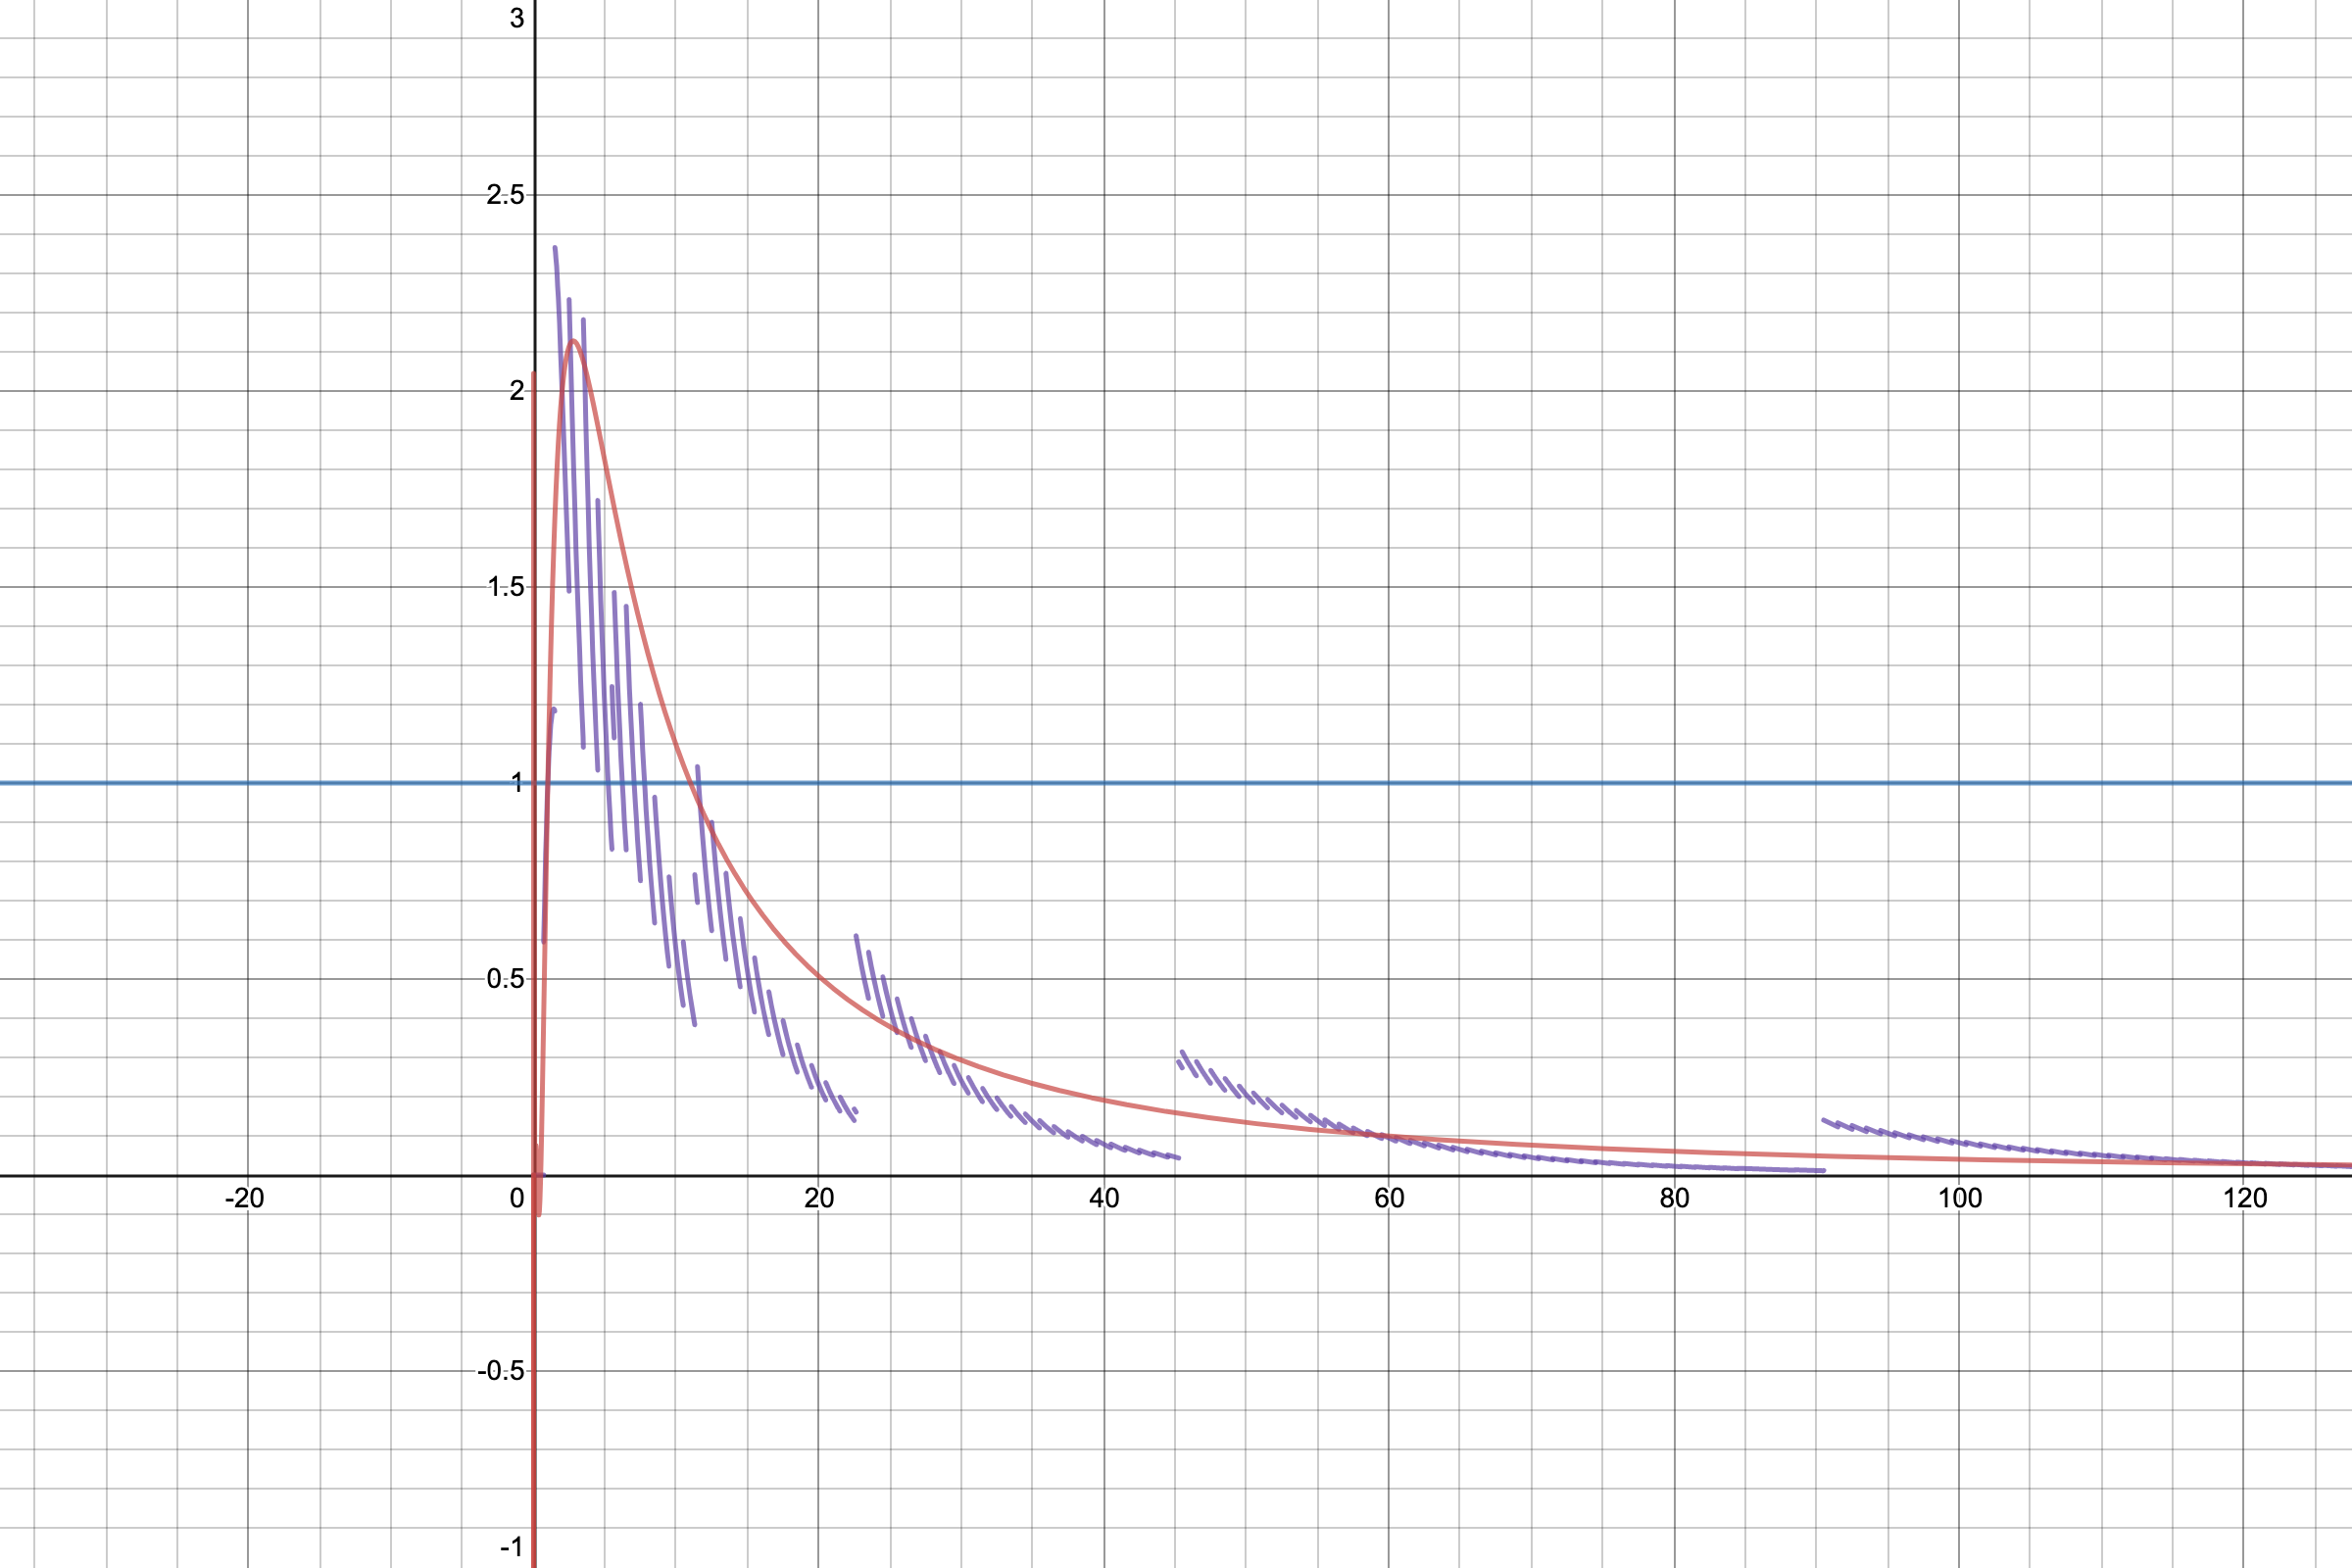
\includegraphics[scale=.2]{graphics/1.2.2.png}}
        \caption{The blue line is $y=1$, the purple line is
        $y=\binom{m}{\log_2 m}/m^{\log_2 m -1}$, and the red line
        is $y = m/(\log_2 m)!$.
        For sufficiently large $m$, the red line and purple lines
        get arbitrarily small.
        The original Desmos plot may be viewed 
        \href{https://www.desmos.com/calculator/64kvnqp8ho}{here}.}
        \label{fig:1.2.2}
    \end{figure}
    
    \item We will take the same approach.
    Define $n = \log_2 m$.
    Let $X_i$ be the indicator random variable that takes value
    1 if and only if all $n$ values of subset $i$ of $[m]$ are all hashed
    to the same value.
    We take the expectation
    \begin{align}
        \E[X] &= \binom{m}{n} \Pr(X_i) \nonumber \\
        &= \frac{m(m-1)(m-1)\dots(m-n+1)}{n!} \frac{1}{m^{n-1}} \nonumber \\
        & \approx \frac{m}{(\log_2 m)!}.
        \nonumber
    \end{align}
    \autoref{fig:1.2.2} shows how $\E[X]$ gets arbitrarily small
    as $m$ increases.
    It follows from Markov's Inequality that, for sufficiently large $m$,
    there is a very low probability of collisions with
    $\log m$ hash tables all of size $O(m)$.
    \qedsymbol
\end{enumerate}   



\newpage
\section*{Problem 3}
\textbf{Collaborators:}  Indu Ramesh.
\medskip

\begin{enumerate}
    \item Set $k=5/\epsilon^2$.
    Define indicator random variable $Y_i$
    that takes value 1 if and only if $X_i$
    comes from the smallest $1/2-\epsilon$
    fraction of $S$.
    Then
    $\E[Y_i] = \E[Y_i^2] =\Pr(Y_i=1) = 1/2-\epsilon$
    by the properties of indicator random variables.
    We now calculate the variance
    \begin{align}
        \Var(Y_i) &= \E[Y_i^2] - \E[Y_i]^2 \nonumber \\
        &=\frac{2-4\epsilon}{4} -
        \frac{1-2\epsilon + \epsilon^2}{4} \nonumber \\
        &= \frac{1-2\epsilon-\epsilon^2}{4}.
        \nonumber
    \end{align}
    Let $Y$ be the sum of $Y_i$.
    By linearity of expectation, $\E[Y] = k/2-k\epsilon$.
    Since the $X_i$ are drawn with replacement,
    the $Y_i$ are independent.
    By linearity of variance for independent variables,
    $\Var(Y) = k(1-2\epsilon-\epsilon^2)/4$.
    
    Observe that $1/2-\epsilon$ of the numbers in $S$
    are less than $\bar{M}$ if and only if the number
    of $X_i$ that come from the smallest $1/2-\epsilon$
    fraction of $S$ is greater than $k/2$.
    Therefore we want to bound
    using Chebyshev's inequality
    \begin{align}
        \Pr(Y > \frac{k}{2}) &=
        \Pr(Y > \frac{k}{2} -k \epsilon + k \epsilon)
        \nonumber \\
        &= \Pr(Y - \left(\frac{k}{2}-k\epsilon\right)>k\epsilon)
        \nonumber \\
        &\leq \Pr(|Y - \E[Y]| \geq k\epsilon)
        \nonumber \\
        &\leq \frac{\Var(Y)}{(k\epsilon)^2} =
        \frac{k-2k\epsilon -k\epsilon^2}{4}\frac{1}{k^2\epsilon^2}
        \nonumber \\
        &< \frac{1}{4k\epsilon^2}
        = \frac{1}{20}
        \nonumber
    \end{align}
    since $k=5/\epsilon^2$ and $\epsilon>0$.
    By symmetry, the probability that more than
    $k/2$ $X_i$ come from the largest $1/2+\epsilon$
    fraction of $S$ is also less than $1/20$.
    Then with probability $9/10$ at least
    $1/2-\epsilon$ numbers in $S$ are smaller
    than $\bar{M}$ and at least 
    $1/2+\epsilon$ numbers in $S$ are larger.
    \qedsymbol
    
    \begin{figure}[H]
        \centering
        \fbox{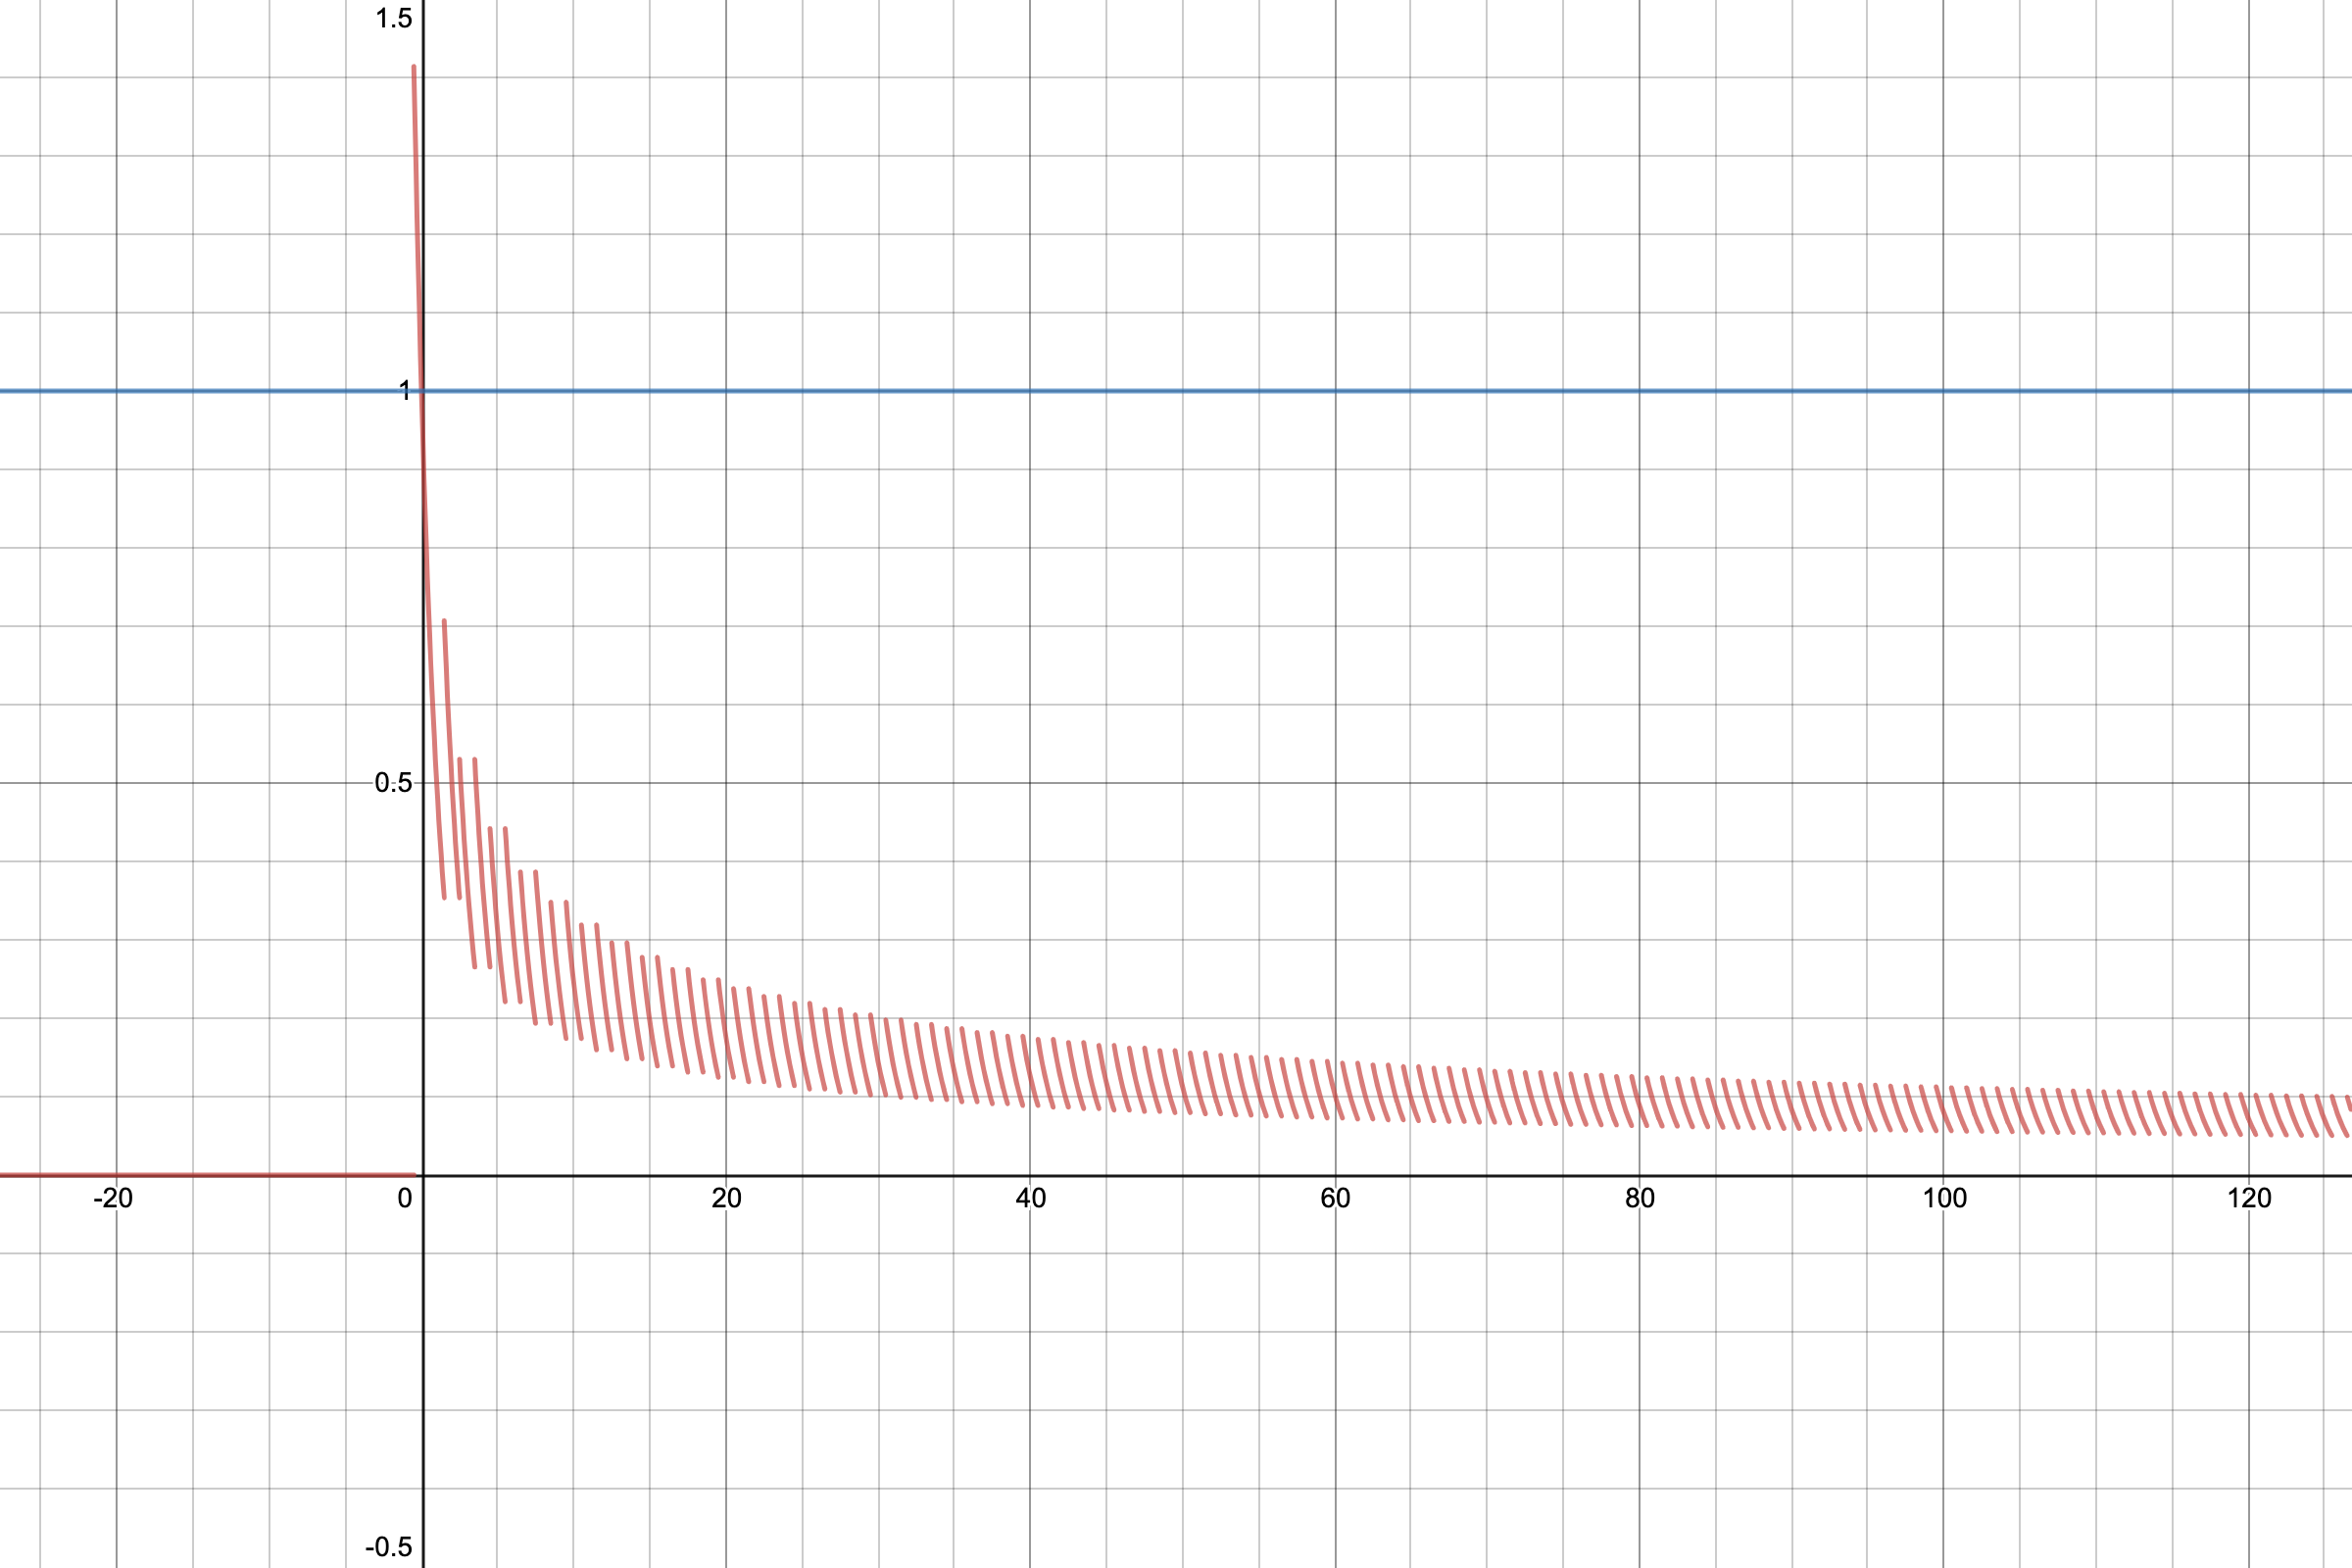
\includegraphics[scale=.2]{graphics/1.3.2.png}}
        \caption{The blue line is $y=1$, and the red line
        is $y = \binom{k}{k/2}1/2^k$.
        For $k>1$, the red line is less than 1 and decreasing.
        The original Desmos plot may be viewed 
        \href{https://www.desmos.com/calculator/zaeb2c8qvf}
        {here}.}
        \label{fig:1.3.2}
    \end{figure}
    
    \item We construct an adversarial $S$
    to show that $o(n)$ samples are not sufficient
    to estimate $M$ within a multiplicative factor
    by $\bar{M}$.
    Let $n$ be even and $S$ a dataset consisting of
    -2 repeated $n/2$ times and 3 repeated $n/2$ times.
    The true median $M$ is 1.
    In a sample of size $k$ when $k$ is odd
    we will only ever have $\bar{M}$ equal to -2 and 3.
    Since neither value is between .5 and 2,
    $k$ must be even for us to have a chance to estimate $M$.
    If the two middle numbers in the sample $X_1,\dots,X_k$
    are -2, we fail.
    If the two middle numbers in the sample are 3,
    we also fail.
    If the two middle numbers in the sample are -2 and 3,
    we succeed.
    So the only way to estimate $M$ within our interval
    is if the sample has exactly as many -2's as 3's.
    The probability of this event is
    \begin{align}
        \binom{k}{k/2} \frac{1}{2}^{k/2} \frac{1}{2}^{k/2}
        = \binom{k}{k/2} \frac{1}{2}^k.
    \nonumber 
    \end{align}
    
    \autoref{fig:1.3.2} demonstrates how this probability
    decreases as $k$ grows.
    So, in fact, the probability of correctly estimating
    $M$ with $\bar{M}$ becomes increasingly unlikely
    for increasing $k$ and any $n$.
    \qedsymbol
    
\end{enumerate}

\newpage
\section*{Problem 4}
\textbf{Collaborators:}  None.
\medskip

\begin{enumerate}
    \item Let $C=\sqrt{nk}$.
    There are two rounds of tests: In the first round,
    we test each group for a total of $\sqrt{nk}$ tests.
    In the second round, we test each group that had a
    positive result. There are $n/\sqrt{nk} = \sqrt{n/k}$
    individuals in a group. In the worst case, each
    individual that is actually positive is in their own group
    so that's a total of $\sqrt{n/k}k = \sqrt{nk}$ more tests.
    Therefore we can identify all positive individuals
    with $2\sqrt{nk}$ tests or fewer.
    \qedsymbol
    
    \item Let $q=\log_2 n$ and $C=4k$.
    Define $A_i$ as the event that COVID-positive
    individual $i$ is in a particular group.
    Since the groups are drawn randomly,
    $P(A_i) = 1/C = 1/4k$.
    Then $P(A_1 \cup \dots \cup A_k) \leq k/4k =1/4$
    by the Union Bound.
    Let $X_i$ be the indicator random variable that COVID-negative
    individual $i$ is in $\log_2 n$ groups that \textit{all}
    test positive for $1 \leq i \leq n$.
    The probability that $X_i=1$ is less than or equal to
    $(1/4)^{\log_2 n}$.
    Now define the total number of false positives
    $X$ as the sum of $X_i$.
    Taking expectation since each event is independent,
    \begin{align}
        \E[X] &= (n-k) \Pr(X_i = 1) \nonumber \\
        &\leq (n-k) (2^{-2})^{\log_2 n} \nonumber \\
        &= \frac{n-k}{n^2} \leq 1/n.
        \nonumber
    \end{align}
    Markov's Inequality yields
    $\Pr(X\geq1) \leq 1/n$.
    Therefore we identify all actual positives and, 
    for $n>10$, we give no false positives with probability
    more than $9/10$.
    \qedsymbol
\end{enumerate}
